\newpage
\section{Frontend}\label{Frontend}
\subsection{Descrizione generale}
\begin{figure}[H]
	\centering
	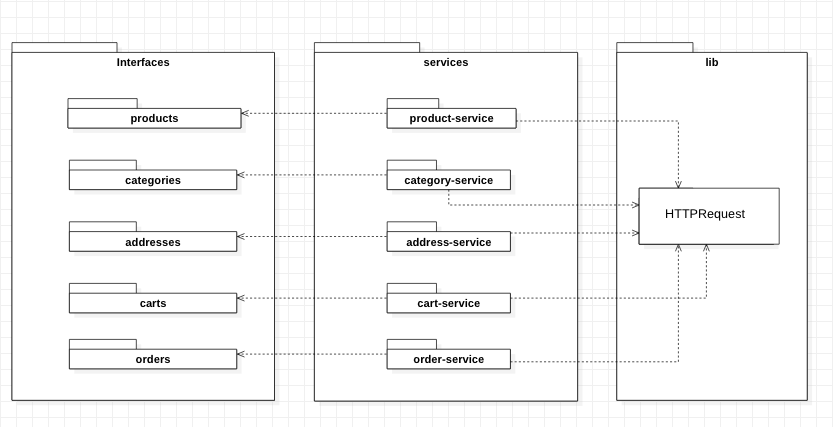
\includegraphics[scale=0.6]{Immagini/Frontend/DiagrammadeiPackage.png}
	\caption{Diagramma dei package}
	\label{fig:fe-packages}
\end{figure}
Il diagramma rappresenta le dipendenze tra le classi che individuano i \glo{microservizi}.
Il package \textbf{interfaces} contiene tutti i tipi che verranno utilizzati dal frontend.
La classe \textbf{HTTPRequest} è stata implementata per centralizzare le chiamate \glo{HTTP} e permettere il controllo dei tipi, consiste in un wrapper della libreria nativa fetch andando a ridefinire i metodi GET, POST, PATCH, PUT e DELETE. Ottiene la variabile d'ambiente contenente l'url del server dal file di configurazione relativo di dotenv, dal costruttore gli verrà passato l'url alla specifica \glo{API} il quale verrà aggiunto all'url precedente e su questo sarà possibile invocare i metodi precedentemente dichiarati.
Il package \textbf{services} rappresenta l'unico punto di collegamento tra i microservizi del backend e il frontend, tramite \glo{API} redatte utilizzando SwaggerHub, i vari servizi al suo interno andranno a invocare HTTPRequest per comunicare con il backend attraverso i metodi definiti.
I microservizi individuati e utilizzati per il frontend sono:
\begin{itemize}
	\item \textbf{Product;}
	\item \textbf{Address;}
	\item \textbf{Categories;}
	\item \textbf{Orders;}
	\item \textbf{Carts.}
\end{itemize}
\subsubsection{Esempio di funzionamento}
Di seguito si riporta il diagramma delle classi relativo al funzionamento del microservizio \textbf{product}. Come si può vedere è presente un'interfaccia ProductService che viene implementata dalla classe ProductServiceFetch e ogni suo metodo istanzia un oggetto HTTPRequest per l'API di interesse. È possibile implementare l'interfaccia ProductService diversamente rispetto a quanto rappresentato senza la necessità di modificare il codice utilizzatore, attraverso la modifica della variabile d'ambiente NEXT\_PUBLIC\_SERVICE\_METHOD sarà possibile scegliere quale implementazione utilizzare altrimenti verrà di default selezionata l'implementazione ProductServiceFetch. 
Per poter procedere con lo sviluppo della parte dei prodotti del frontend parallelamente con il backend, lo sviluppatore ha a disposizione la classe ProductServiceMock la quale ritornerà i dati predefiniti senza dover richiamare il server, basterà impostare la variabile NEXT\_PUBLIC\_SERVICE\_METHOD="mock".
\begin{figure}[H]
	\centering
	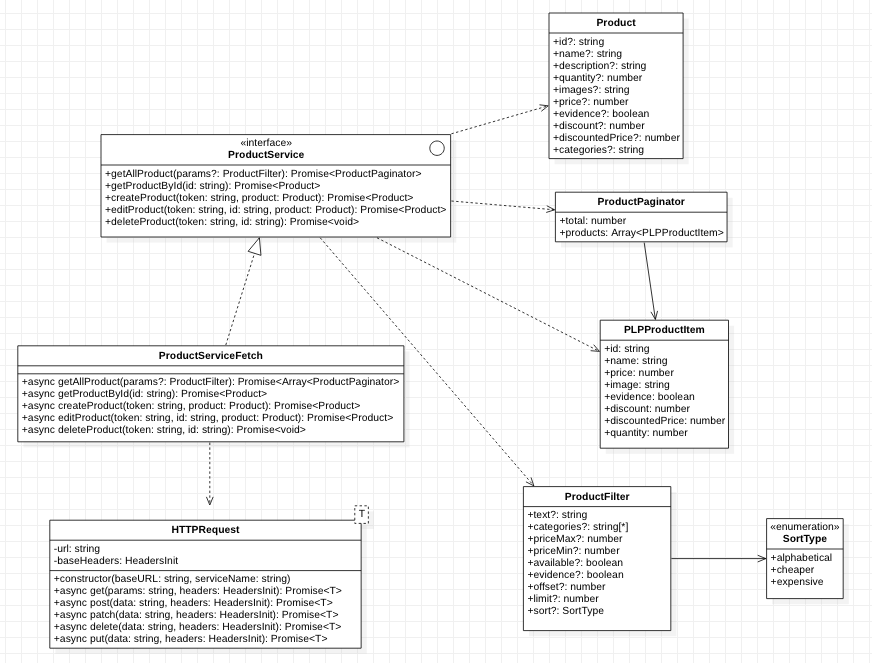
\includegraphics[width=\textwidth]{Immagini/Frontend/ProductService.png}
	\caption{Microservizio Product}
	\label{fig:fe-productservice}
\end{figure}

